\documentclass[unicode,12pt,aspectratio=169,dvipdfmx]{beamer}
\usepackage{bxdpx-beamer}
\usetheme[progressbar=frametitle]{metropolis}
\renewcommand{\kanjifamilydefault}{\gtdefault}
\usepackage{bm}

\title{介護における音響HARと連合学習を用いた異常検知}
% \title{「A Survey on Federated Learning in Human Sensing」について}
\author{竹本志恩}
\institute{INIAD}
\date{\today}
\subject{研究報告 / 輪読}
\AtBeginSection[]{
  \begin{frame}[plain]
    \frametitle{目次}
    \tableofcontents[currentsection, hideallsubsections]
  \end{frame}
}

% --- セクション開始時に目次を表示 ---
\AtBeginSection[]{%
  \frame{\frametitle{目次}\tableofcontents[currentsection, hideallsubsections]}%
}

\begin{document}

% タイトルスライド
\begin{frame}
    \titlepage
\end{frame}

% 各セクション
\section{はじめに}
\begin{frame}{はじめに}
    \begin{itemize}
        \item 発表論文の概要
        \begin{itemize}
            \item タイトル: A Survey on Federated Learning in Human Sensing
            \item 著者: Mohan Li, Martin Gjoreski, Pietro Barbiero, Gašper Slapničar, Mitja Luštrek, Nicholas D. Lane, Marc Langheinrich
            \item 出典: ACM, 2025年1月公開
            \item 内容: \textbf{Human Sensing分野におけるFederated Learning (FL) の応用}に関する包括的サーベイ。現状、課題、分類、今後の研究方向を提示。
        \end{itemize}
    \end{itemize}
\end{frame}


\begin{frame}{はじめに}
    \begin{itemize}
        \item Human Sensingとは
        \begin{itemize}
            \item 人の活動、生理/心理状態などを監視し、生活の質向上に貢献
            \item 以下で進展:
            \begin{itemize}
                \item センサ技術の発展
                \item ウェアラブルデバイスの普及
            \end{itemize}
            \item 用いるデータはプライバシで、法や倫理的な懸念が存在
        \end{itemize}
        \item プライバシの観点で、FLの応用が考えられる
    \end{itemize}
\end{frame}



\section{本サーベイの貢献と主要ドメイン}
\begin{frame}{本サーベイの貢献}
    \begin{itemize}
        \item Human SensingにおけるFLの包括的サーベイ
        \begin{itemize}
            \item 既存のFLサーベイはIoTや医療(IoMT)、推薦システムに焦点
            \item \textbf{本サーベイはHuman Sensingに特化}
        \end{itemize}
        \item FLの応用評価のための\textbf{8次元フレームワーク}を提案
        \begin{itemize}
            \item プライバシーとセキュリティ、通信コスト、システム異質性
            \item 統計的異質性、ラベルなしデータ使用、簡略化された実験設定
            \item サーバ $|$ クライアント最適化FL
        \end{itemize}
        \item 応用指向の分類を提示
    \end{itemize}
\end{frame}

\begin{frame}{主要な応用ドメイン}
    \begin{columns}
        \begin{column}[T]{.6\linewidth}
            \begin{itemize}
                \item Human SensingにおけるFLを6つに分類
                \item \textbf{Activity Recognition (HAR) が最多の分野}
                \begin{itemize}
                    \item サーベイ対象論文の\textbf{31.6\%}
                    \item Well-being (21.4\%)、User Identification (15.3\%)...
                    \item Interface Development は最少(3.3\%)
                \end{itemize}
                \item \textbf{HARは注目される応用先}
            \end{itemize}
        \end{column}
        \begin{column}[T]{.4\linewidth}
            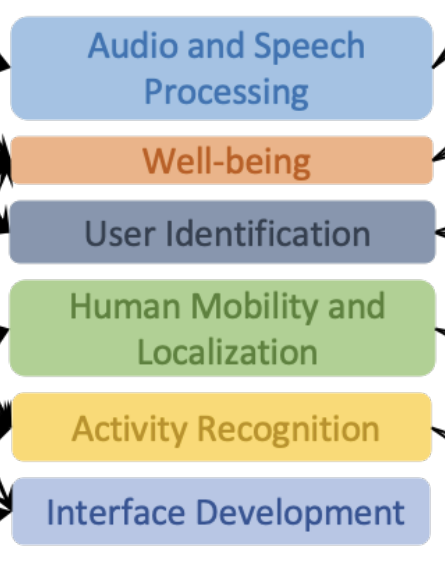
\includegraphics[scale=0.6]{figures/対象の分野.png}                    
        \end{column}
    \end{columns}
    \end{frame}

\begin{frame}{Fig.5}
    \center 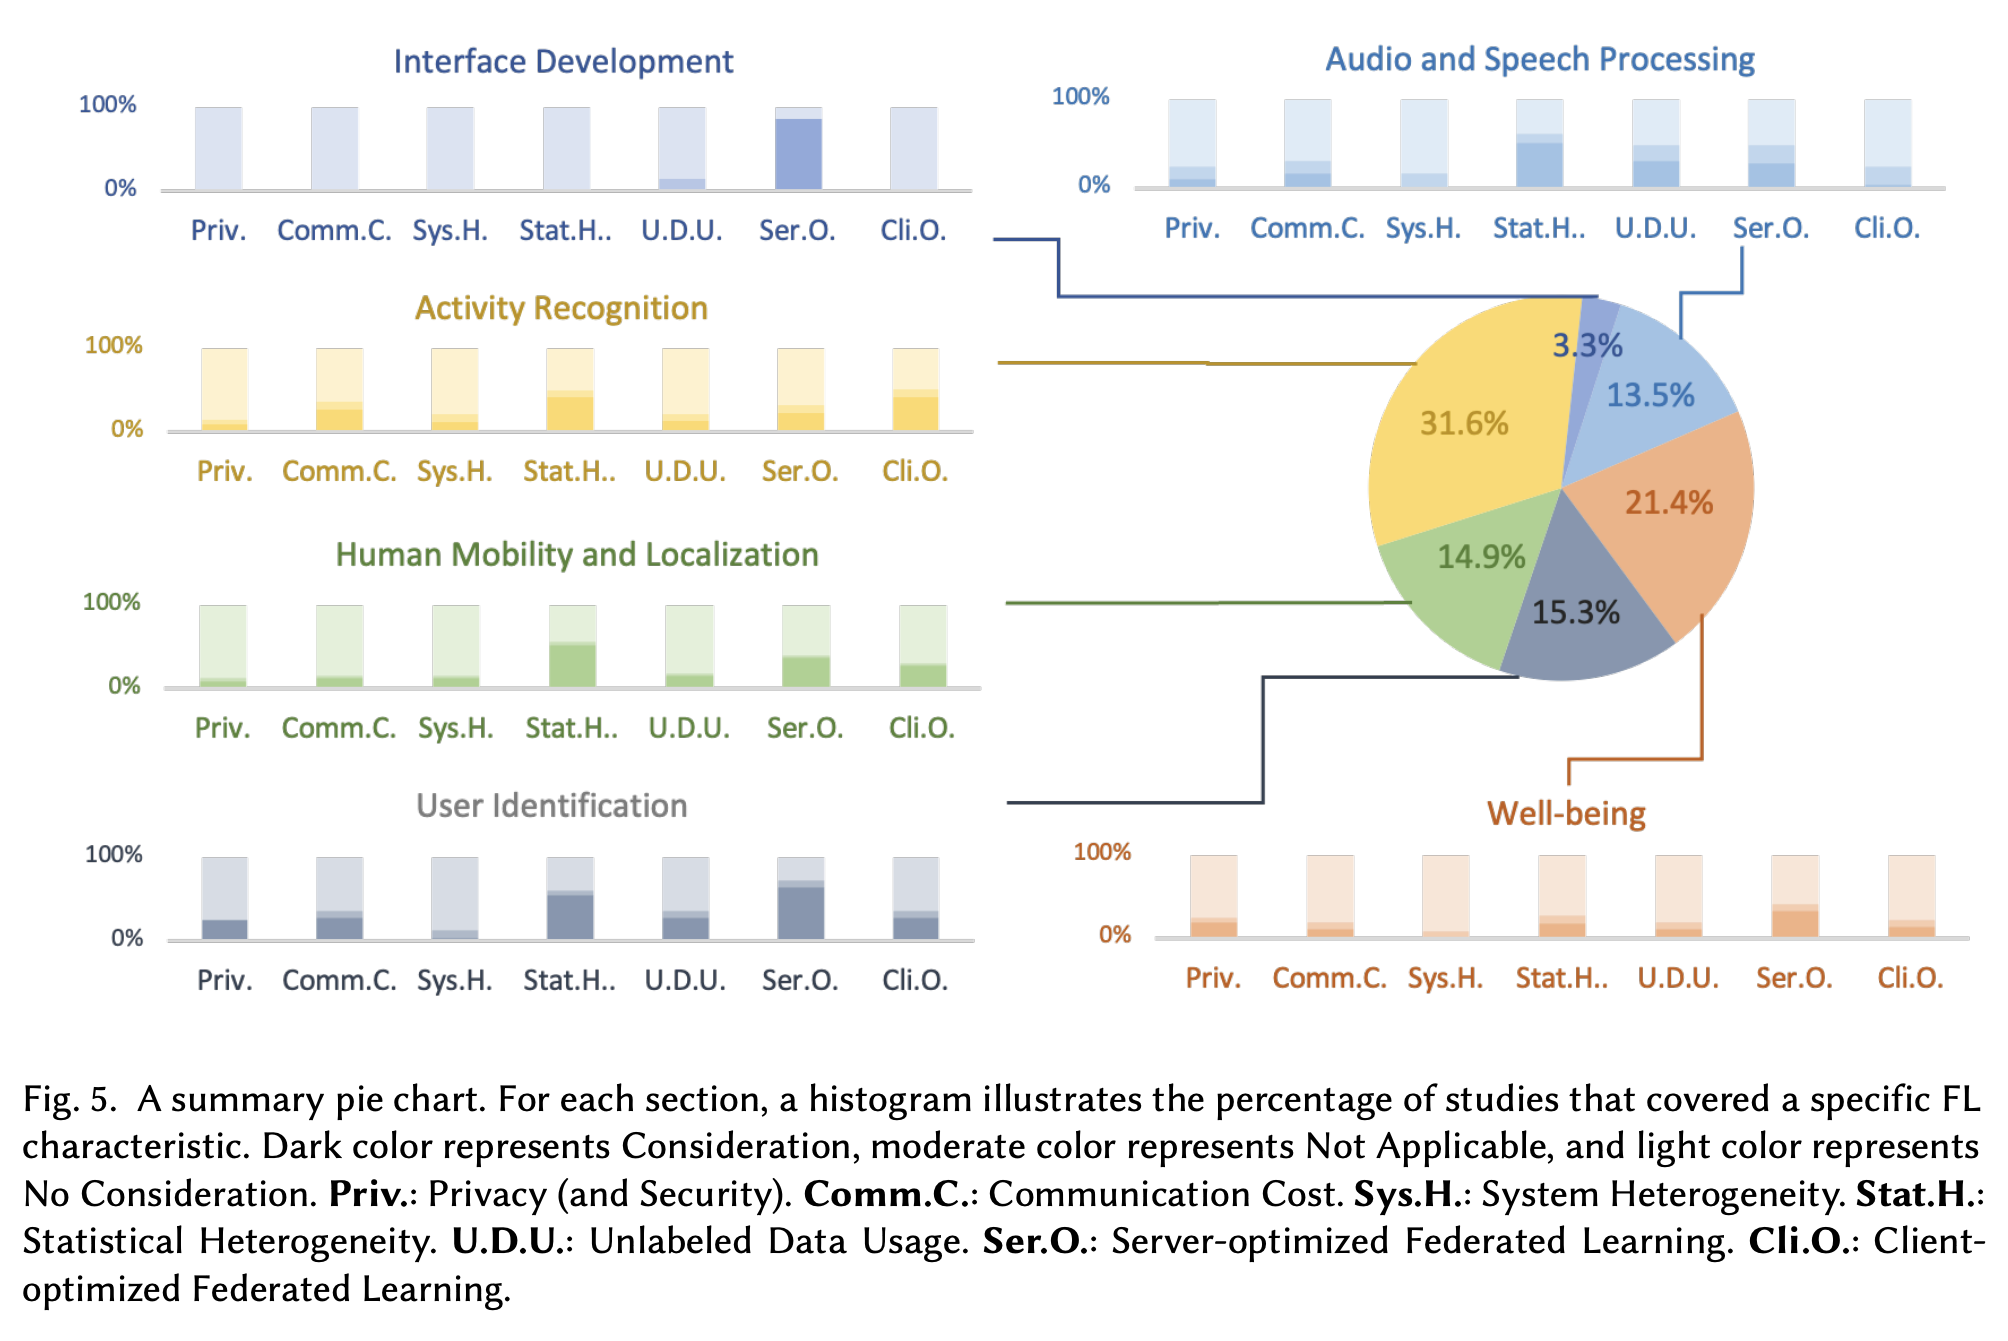
\includegraphics[scale=0.3]{figures/domain_per.png}                    
\end{frame}


\section{Human Activity Recognition (HAR) とは}
\begin{frame}{Human Activity Recognition (HAR) とは}
    \begin{itemize}
        \item HARの定義と応用
        \begin{itemize}
            \item センサの値から\textbf{人の活動を認識}する問題
            \item ヘルスケア、スマートホーム、リハビリテーション、転倒検知など
        \end{itemize}
        \item 主要なセンサ
        \begin{itemize}
            \item \textbf{ウェアラブルセンサ}
                \begin{itemize}
                    \item スマートウォッチ、スマートフォン、リストバンド
                    \item 加速度、ジャイロスコープなど
                    \item 小型、低コスト、柔軟な装着が可能。
                \end{itemize}
            \item \textbf{環境センサ}
                \begin{itemize}
                    \item マイク、圧力センサなど
                    \item ユーザの負担が少ない
                \end{itemize}
            \item \textbf{カメラ系}: ビデオや画像、直接的で正確な情報を提供
        \end{itemize}
    \end{itemize}
\end{frame}


\begin{frame}{Human Activity Recognition (HAR) とは}
    \begin{itemize}
        \item HARの課題
        \begin{itemize}
            \item \textbf{プライバシー懸念}
                \begin{itemize}
                    \item カメラの情報量の多さ
                    \item 中央集権的なデータ
                    % データ最小限の原則を守れない
                \end{itemize}
            \item \textbf{通信コスト}: 大量のデータで負担
            % \item \textbf{手作業による特徴エンジニアリング}: 従来のML手法ではドメイン知識に依存し、時間と労力がかかる。
            \item \textbf{限られたデータセット}: プライバシー懸念から大規模な実世界データセットが少ない
        \end{itemize}
    \end{itemize}
\end{frame}



\section{HARにおけるFLの導入と想定シナリオ}
\begin{frame}{HARにおけるFLの導入}
    \begin{itemize}
        \item FLによる課題解決の方向性
        \begin{itemize}
            \item \textbf{プライバシー保護}: モデルの更新情報のみを共有
            \item \textbf{通信コスト削減}: モデル更新情報が生データより小さければ可能
            \item \textbf{分散型学習}: 一箇所に収集・転送・保存する必要がない
        \end{itemize}
        \item HARにおけるFL研究の活発化
        \begin{itemize}
            \item サーベイ論文でも多くが集中
            \item \textbf{現実世界の複雑な課題} (Non-IIDなど)の対応が検討
        \end{itemize}
    \end{itemize}
\end{frame}

\begin{frame}{HAR-FL想定シナリオ:介護施設での見守りシステム}
    \begin{itemize}
        \item 目的
        \begin{itemize}
            \item 異常を早期に検知し、介護者に通知
            \item 緊急性の高いイベントを検知
            \item 特に、転倒、異様な咳き込み、苦痛の声など
        \end{itemize}
        \item 背景
        \begin{itemize}
            \item 高齢化社会における介護人材不足の深刻化
            \item 安価で効果的な見守りシステムの需要
        \end{itemize}
    \end{itemize}
\end{frame}

\begin{frame}{HAR-FL想定シナリオ:介護施設での見守りシステム}
    \begin{itemize}
        \item 使用技術
        \begin{itemize}
            \item \textbf{音によるHAR}
            \begin{itemize}
                \item 各部屋のIoTデバイスで環境音を収集
                \item 音響イベントを検出
            \end{itemize}
            \item \textbf{行動認識}
            \begin{itemize}
                \item 利用者の行動(転倒、呼吸困難など)を判断
                \item 音響イベントや、時系列などの傾向が材料
            \end{itemize}
            \item \textbf{Federated Learning (FL)}
            \begin{itemize}
                \item 各部屋のIoTデバイスがクライアント
                % \item モデルを学習・更新
            \end{itemize}
        \end{itemize}
    \end{itemize}
\end{frame}



\begin{frame}{HAR-FL想定シナリオ:介護施設での見守りシステム}
    \begin{itemize}
        \item FL導入の利点
        \begin{itemize}
            \item プライバシー保護
            \begin{itemize}
                \item 生データを部屋内で処理
                \item 漏洩リスクを低減
            \end{itemize}
            \item{パーソナル化}
            \begin{itemize}
                \item 各部屋の環境や利用者の生活パターンに合わせた
                \item モデルを学習し、精度向上。
            \end{itemize}
            % \item {スケーラビリティ}: クライアント(部屋)が増えても対応しやすい分散学習。
            % ..?ここは微妙
        \end{itemize}
    \end{itemize}
\end{frame}


\begin{frame}{想定される課題と検討}
    \begin{itemize}
        \item \textbf{緊急性の高いイベントデータの収集とアノテーション}:
        \begin{itemize}
            \item これらのデータは稀で、収集・準備に課題。
            \item オープンデータ(SAFE, DESED, AudioSetなど)の活用や合成データ生成などの検討。
        \end{itemize}
        \item \textbf{データ異質性 (Non-IID)}:
        \begin{itemize}
            \item 部屋ごと、利用者ごとに発生する音響イベントの種類や頻度、音響特性が異なる。
            \item クライアントごとのデータ分布のばらつきに対応が必要。
        \end{itemize}
        \item \textbf{クライアントの異質性}:
        \begin{itemize}
            \item IoTデバイスの計算能力、メモリ、接続性などが異なる 
            % 従来はそう 統一すれば一旦無視できるはず
            \item 軽量なモデルや連合分割学習(FSL)などが有効。
        \end{itemize}
    \end{itemize}
\end{frame}

\begin{frame}{想定される課題と検討事項}
    \begin{itemize}
        \item \textbf{リアルタイム性能}:
        \begin{itemize}
            \item 異常検知には即時性が大切
            \item FLの学習・推論プロセス全体のレイテンシ検討
        \end{itemize}
        \item \textbf{モデルの汎化}:
        \begin{itemize}
            \item 特定の環境で学習したモデルが、別の部屋や新規利用者に適用できるか
            \item メタ学習や表現学習を用いたアプローチが有望
        \end{itemize}
    \end{itemize}
\end{frame}



\section{HAR-FLの主要課題とFLの対応(サーベイより)}
\begin{frame}{HAR-FLにおける主要な課題とFLの対応}
    \begin{itemize}
        \item \textbf{データ異質性 (Non-IID)}
        \begin{itemize}
            \item 課題: クライアント間で活動タイプやセンサーデータ(信号分布)に大きな偏りがある。従来のFedAvgでは性能が劣化しやすい。
            \item FLによる対応例: \textbf{パーソナル化FL (pFL)} (Meta-HAR 、FedDL )、クラスタリング 、知識蒸留 。
        \end{itemize}
        \item \textbf{限られたラベルデータ/ラベルなしデータ}
        \begin{itemize}
            \item 課題: ラベル付けのコストや希少なイベントのため、十分なラベル付きデータがない。
            \item FLによる対応例: \textbf{半教師あり学習} 、教師なし学習 、自己教師あり学習 。
        \end{itemize}
        \item \textbf{通信コスト}
        \begin{itemize}
            \item 課題: エッジデバイスの帯域幅やバッテリーの制約。
            \item FLによる対応例: \textbf{動的レイヤー共有 (FedDL)} 、モデル圧縮・量子化 。
        \end{itemize}
    \end{itemize}
\end{frame}

\begin{frame}{HAR-FLにおける主要な課題とFLの対応 (続き)}
    \begin{itemize}
        \item \textbf{プライバシー/セキュリティ}
        \begin{itemize}
            \item 課題: FLでも勾配からの情報漏洩やポイズニング攻撃などのリスク。
            \item FLによる対応例: \textbf{差分プライバシー (DP)} 、\textbf{セキュアアグリゲーション} 、クライアントフィルタリング 、連合分割学習(FSL)。
        \end{itemize}
        \item \textbf{システム異質性}
        \begin{itemize}
            \item 課題: クライアントデバイスの計算能力、メモリ、接続性などが異なる。
            \item FLによる対応例: リソースアウェアなクライアント選択や学習手法。
        \end{itemize}
    \end{itemize}
\end{frame}

\section{まとめ}
\begin{frame}{まとめ}
    \begin{itemize}
        \item Human Sensingは\textbf{データプライバシが課題}
        \item Federated Learningは\textbf{解決策}として有望
        \item Human Activity Recognition (HAR) 分野は、FLの応用が活発
    \end{itemize}
\end{frame}

\begin{frame}{まとめ}
    \begin{itemize}
        \item \textbf{介護施設での見守りシステム}のシナリオでHAR-FLは
        \begin{itemize}
            \item プライバシーを保護しつつ
            \item \textbf{利用者個人に合わせた高精度な異常検知}の可能性
        \end{itemize}
        \item 展望
        \begin{itemize}
            \item より現実的な条件下での性能評価
            \item 多様なモダリティの統合
            \item プライバシ保護技術の発展
            \item HAR-FLの\textbf{社会実装を加速}させることが期待される。
        \end{itemize}
    \end{itemize}
\end{frame}


\end{document}